\subsection{Beam Monitoring}
\label{sec:beam_mon}

Helicity-correlations in the beam properties such as energy and position are
a primary concern for parity-violation experiments.  
At Jefferson Lab, the beam position is measured by ``stripline"
monitors~\cite{stripline}, each of which consists of a set of four thin wires
placed symmetrically around the beam pipe. The wires act as antennae
that provide a signal (modulated by the microwave structure of the
electron beam) proportional to the beam position as well as
intensity. Figure~\ref{fig5:jlabcorr} shows the correlation between
the measured position at a BPM near the target compared with the
predicted position using neighboring BPMs for a beam current of
100 $\mu$A ($2\times 10^{13}$ electrons per window). A precision
for $\delta(\Delta X_i)$ close to 1 $\mu$m was obtained for the
average beam position for a beam window containing $2\times
10^{13}$ electrons.

\begin{figure}[tb]
\begin{center}
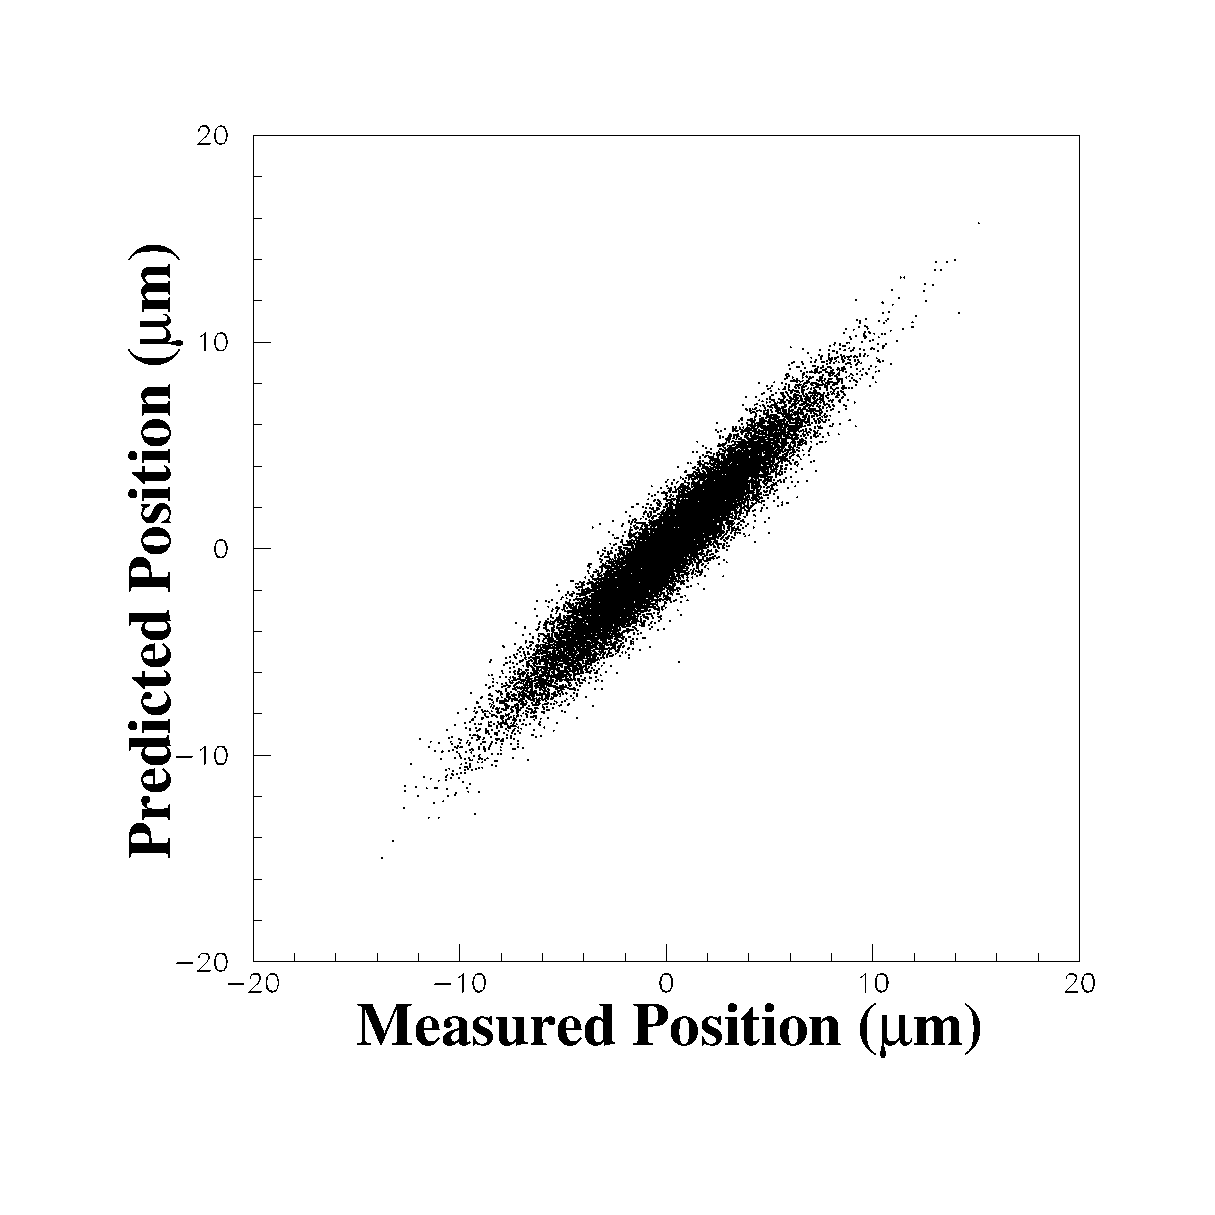
\includegraphics[width=3.6in]{RM/fig5_ycorrbw.eps}
\caption{Window-to-window beam jitter as measured
by a BPM is 
plotted along the $x$ axis. On the $y$ axis is plotted the beam
position as predicted by nearby BPMs. The residuals are smaller
than 1 $\mu$m.}
\label{fig5:jlabcorr}
\end{center}
\end{figure}

To measure the beam intensity, microwave cavity BCMs have been
developed at Jefferson Lab~\cite{A-NIM}. The precision $\delta(\asy_I)$ that has
been achieved for a 30 ms beam window at 100 $\mu$A is $4\times
10^{-5}$. This superior resolution is a 
result of good radiofrequency (rf)
instrumentation as well as a high resolution 18-bit ADC, which
will be discussed in section \ref{sec:daq}.

Let the detected scattered flux of electrons be $D$ in each spectrometer,
and the beam current $I$,
measured independently for every window
by integrating the signals over the helicity period.  From these 
we obtained the normalized flux $d_i \equiv D_i/I_i$ and 
the cross section asymmetry $(A_d)_i$ for the
$i$th window pair. The raw asymmetry was then obtained by
appropriate averaging of $N$ measurements:
%
\begin{eqnarray} \label{eq:asyraw}
(A_d)_i & \equiv &
{\left(\frac{d^+-d^-}
{d^++d^-}\right)}_i 
\equiv {\left(\frac{\Delta d}
{2d}\right)}_i 
\nonumber \\
\quad \delta(\asy_d) & = &
\sigma(\asy_d)/\sqrt{N}. \label{eqn:pulsepair}
\end{eqnarray}
%
where $+$ and $-$ denote the two helicity states in a pair.

A major goal of the experimental design is to $\sigma(\asy_d)$ should be
dominated by the counting statistics in the scattered flux.
As shown by fig N in ref ~\cite{pvdis_nim}, this goal was met.

There are two key parameters for each experimentally measured
quantity $M$, such as detector rate, beam intensity, or beam position. 
The first is $\sigma(\Delta M)$, the size of the relative window pair-to-window pair
fluctuations in $\Delta M\equiv M_{+} - M_{-}$, which is affected by
real fluctuations in the electron flux. The second is
$\delta(\Delta M)$, the relative accuracy with which the window
pair differences in $M$ can be measured compared to the true
value, which is dominated by instrumentation noise.

If $\sigma(\Delta M)$ is large enough, it might mean that there
are non-statistical contributions to $\sigma(\asy_d)$ so that the
latter is no longer dominated by counting statistics. In this
case, it is crucial that $\delta(\Delta M)\ll\sigma(\Delta M)$ so
that window pair to window pair corrections for the fluctuations
in $\Delta M$ can be made.

As stated in \ref{sec:beam_fluc}, we desire that
$\sigma(\asy_d)$ be dominated by counting statistics.
An example of possible non-statistical contributions
is window-to-window relative beam intensity
fluctuations, $\sigma(A(I)) \equiv \sigma(\Delta I/2I)$,
which were observed to vary between $2\times 10^{-4}$ and
$2\times 10^{-3}$, depending on the quality of the laser and the
beam tune. This is remarkable and a unique feature of the beam at
Jefferson lab, since $\sigma(\asy_I)<\sigma(\asy_d)$. Nevertheless, the
detector-intensity correlation can be exploited to remove the
dependence of beam charge fluctuations on the measured asymmetry:
\begin{equation}
(\asy_d)_i \simeq
\left(\frac{\Delta D}{2D} - \frac{\Delta I}{2I}\right)_i \equiv
(\asy_D - \asy_I)_i.
\end{equation}
(This is equation \ref{eq:asyraw}
to first order.)

Similarly, $\sigma(\asy_d)$ might be affected by random beam
fluctuations in energy, position and angle. The corrections can be
parameterized as follows:
\begin{equation}
(\acorr_d)_i = \left(\frac{\Delta D}{2D} - \frac{\Delta I}{2I}\right)_i
-\sum_j{\left( {\alpha_j(\Delta X_j)_i}\right)}.
\end{equation}
Here, $X_j$ are beam parameters such as energy, position and
angle and $\alpha_j \equiv \partial D/\partial X_j$ are
coefficients that depend on the kinematics of the specific
reaction being studied, as well as the detailed spectrometer and
detector geometry of the experiment.

By judicious choices of beam position monitoring devices (BPMs)
and their respective locations, several measurements of beam
position can be made from which the average relative energy,
position, and angle of approach of each ensemble of electrons in a
helicity window on target can be inferred. One can then write
\begin{equation} 
(\acorr_d)_i = \left(\frac{\Delta D}{2D} - \frac{\Delta I}{2I}\right)_i
-\sum_j{\left({\beta_j(\Delta M_j)_i}\right)}.
\end{equation}
Here $M_i$ are a set of 5 BPMs that span the parameter space of
energy, position, and angle on target, and $\beta_i \equiv \partial
D/\partial M_i$. It is worth noting that this approach of making
corrections window by window automatically accounts for occasional
random instabilities in the accelerator (such as klystron
failures) that are characteristic of normal running conditions.

During our experiment run, we found that $\sigma(\Delta M_j)$ varied
between 1 and 10 $\mu$m and $\sigma (\asy_E)$ was typically less
than $10^{-5}$. These fluctuations were small enough that their
impact on $\sigma (\asy_d)$ was negligible. Indeed, we believe that a
significant contribution to the fluctuations in each monitor
difference $\Delta M$ was the intrinsic measurement precision
$\delta(\Delta M_i)$. We elaborate on this in section
~\ref{sec:beam_mon},
where we discuss the monitoring instrumentation.

Another important consideration is the accuracy with which the
coefficients $\beta_i$ are measured. As mentioned earlier, these
coefficients were evaluated using beam modulation, and will be
discussed in Sect.~\ref{bmod}.

The above discussion regarding measurement accuracy and its impact
on $\sigma(\asy_d)$ is particularly relevant in the monitoring of the
electron beam properties such as beam intensity, trajectory and
energy.
